\documentclass[a4paper]{article}
\usepackage{student}

% Metadata
\date{\today}
\setmodule{CS110: Computer Architecture}
\setterm{Spring, 2024}

%-------------------------------%
% Other details
% DONE: Fill these
%-------------------------------%
\title{Assignment 4: Digital circuit}
\setmembername{Renyi Yang}  % Fill student name
\setmemberuid{2023533030}  % Fill  student id

%-------------------------------%
% Add / Delete commands and packages
% DONE: Add / Delete here as you need
%-------------------------------%
\usepackage{amsmath,amssymb,bm}
\usepackage{hyperref}
\usepackage{float}
\usepackage{tikz}

\newcommand{\KL}{\mathrm{KL}}
\newcommand{\R}{\mathbb{R}}
\newcommand{\E}{\mathbb{E}}
\newcommand{\T}{\top}

\newcommand{\expdist}[2]{%
        \normalfont{\textsc{Exp}}(#1, #2)%
    }
\newcommand{\expparam}{\bm \lambda}
\newcommand{\Expparam}{\bm \Lambda}
\newcommand{\natparam}{\bm \eta}
\newcommand{\Natparam}{\bm H}
\newcommand{\sufstat}{\bm u}

% Main document
\begin{document}
% Add header
\header{}
\textcolor{red}{\textbf{Attention: }}
\textbf{Recommend using \LaTeX \space to complete your work. You can use any tool, such as Logisim, Visio, Draw.io, PowerPoint, etc., to create diagrams. However, handwritten or hand-drawn content is not acceptable.}

\section{Combinational logic}
The circuit shown in Figure.~\ref{fig:Q1_circuit} is a 1-bit comparator. Answer the following questions. \\

\begin{figure}[htbp]
    \centering
    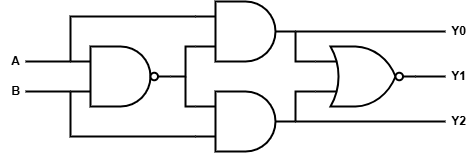
\includegraphics[width=0.8\textwidth]{Q1_circuit.png}
    \caption{A 1-bit comparator circuit}
    \label{fig:Q1_circuit}
\end{figure}

(a) Write the un-simplified logic expressions for $Y0$, $Y1$ and $Y2$. \textbf{[6 pt]}

(b) Draw the truth table of this circuit in the following table.\textbf{[6 pt]}

(c) Write the sum of minterm for $Y0$, $Y1$ and $Y2$. \textbf{[6 pt]}

(d) What comparison do the outputs $Y0$, $Y1$ and $Y2$ represent respectively? e.g: $Y0=1$ represents $A=B$, $A<B$ or $A>B$ (one of the three cases). \textbf{[6 pt]}

(e) Draw the circuit of an unsigned 2-bit comparator using this 1-bit comparator and the following logic gates: 2-input AND, 2-input OR, and 1-input NOT. The 2-bit comparator has two 2-bit inputs $A1A0$ and $B1B0$, three outputs $Y0$, $Y1$ and $Y2$ with the same function as the 1-bit comparator. You can use the 1-bit comparator as a basic logic block as shown in Figure.~\ref{fig:Q1_comparator_1}. \textbf{[10 pt]}
\begin{figure}[htbp]
    \centering
    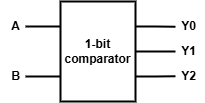
\includegraphics[width=0.4\textwidth]{Q1_comparator_1.png}
    \caption{A 1-bit comparator diagram}
    \label{fig:Q1_comparator_1}
\end{figure}
\begin{answer}[Question 1]
    (a)
    $$Y0 = A \cdot \overline{AB}$$
    $$Y1 = \overline{A \cdot \overline{AB} + B \cdot \overline{AB}}$$
    $$Y2 = B \cdot \overline{AB}$$

    (b) Do not modify the given values in the truth table.\\
    \begin{center}
        \begin{tabular}{ |c|c||c|c|c| }
            \hline
            A & B & Y2 & Y1 & Y0 \\
            \hline
            0 & 0 & 0  & 1  & 0  \\
            \hline
            0 & 1 & 1  & 0  & 0  \\
            \hline
            1 & 0 & 0  & 0  & 1  \\
            \hline
            1 & 1 & 0  & 1  & 0  \\
            \hline
        \end{tabular}
    \end{center}

    (c)
    $$Y0 = A \cdot \overline{B}$$
    $$Y1 = AB + \overline{A} \cdot \overline{B}$$
    $$Y2 = B \cdot \overline{A}$$

    (d) $Y0=1$ represents $A>B$, $Y1=1$ represents $A=B$, and $Y2=1$ represents $A<B$

    (e)

    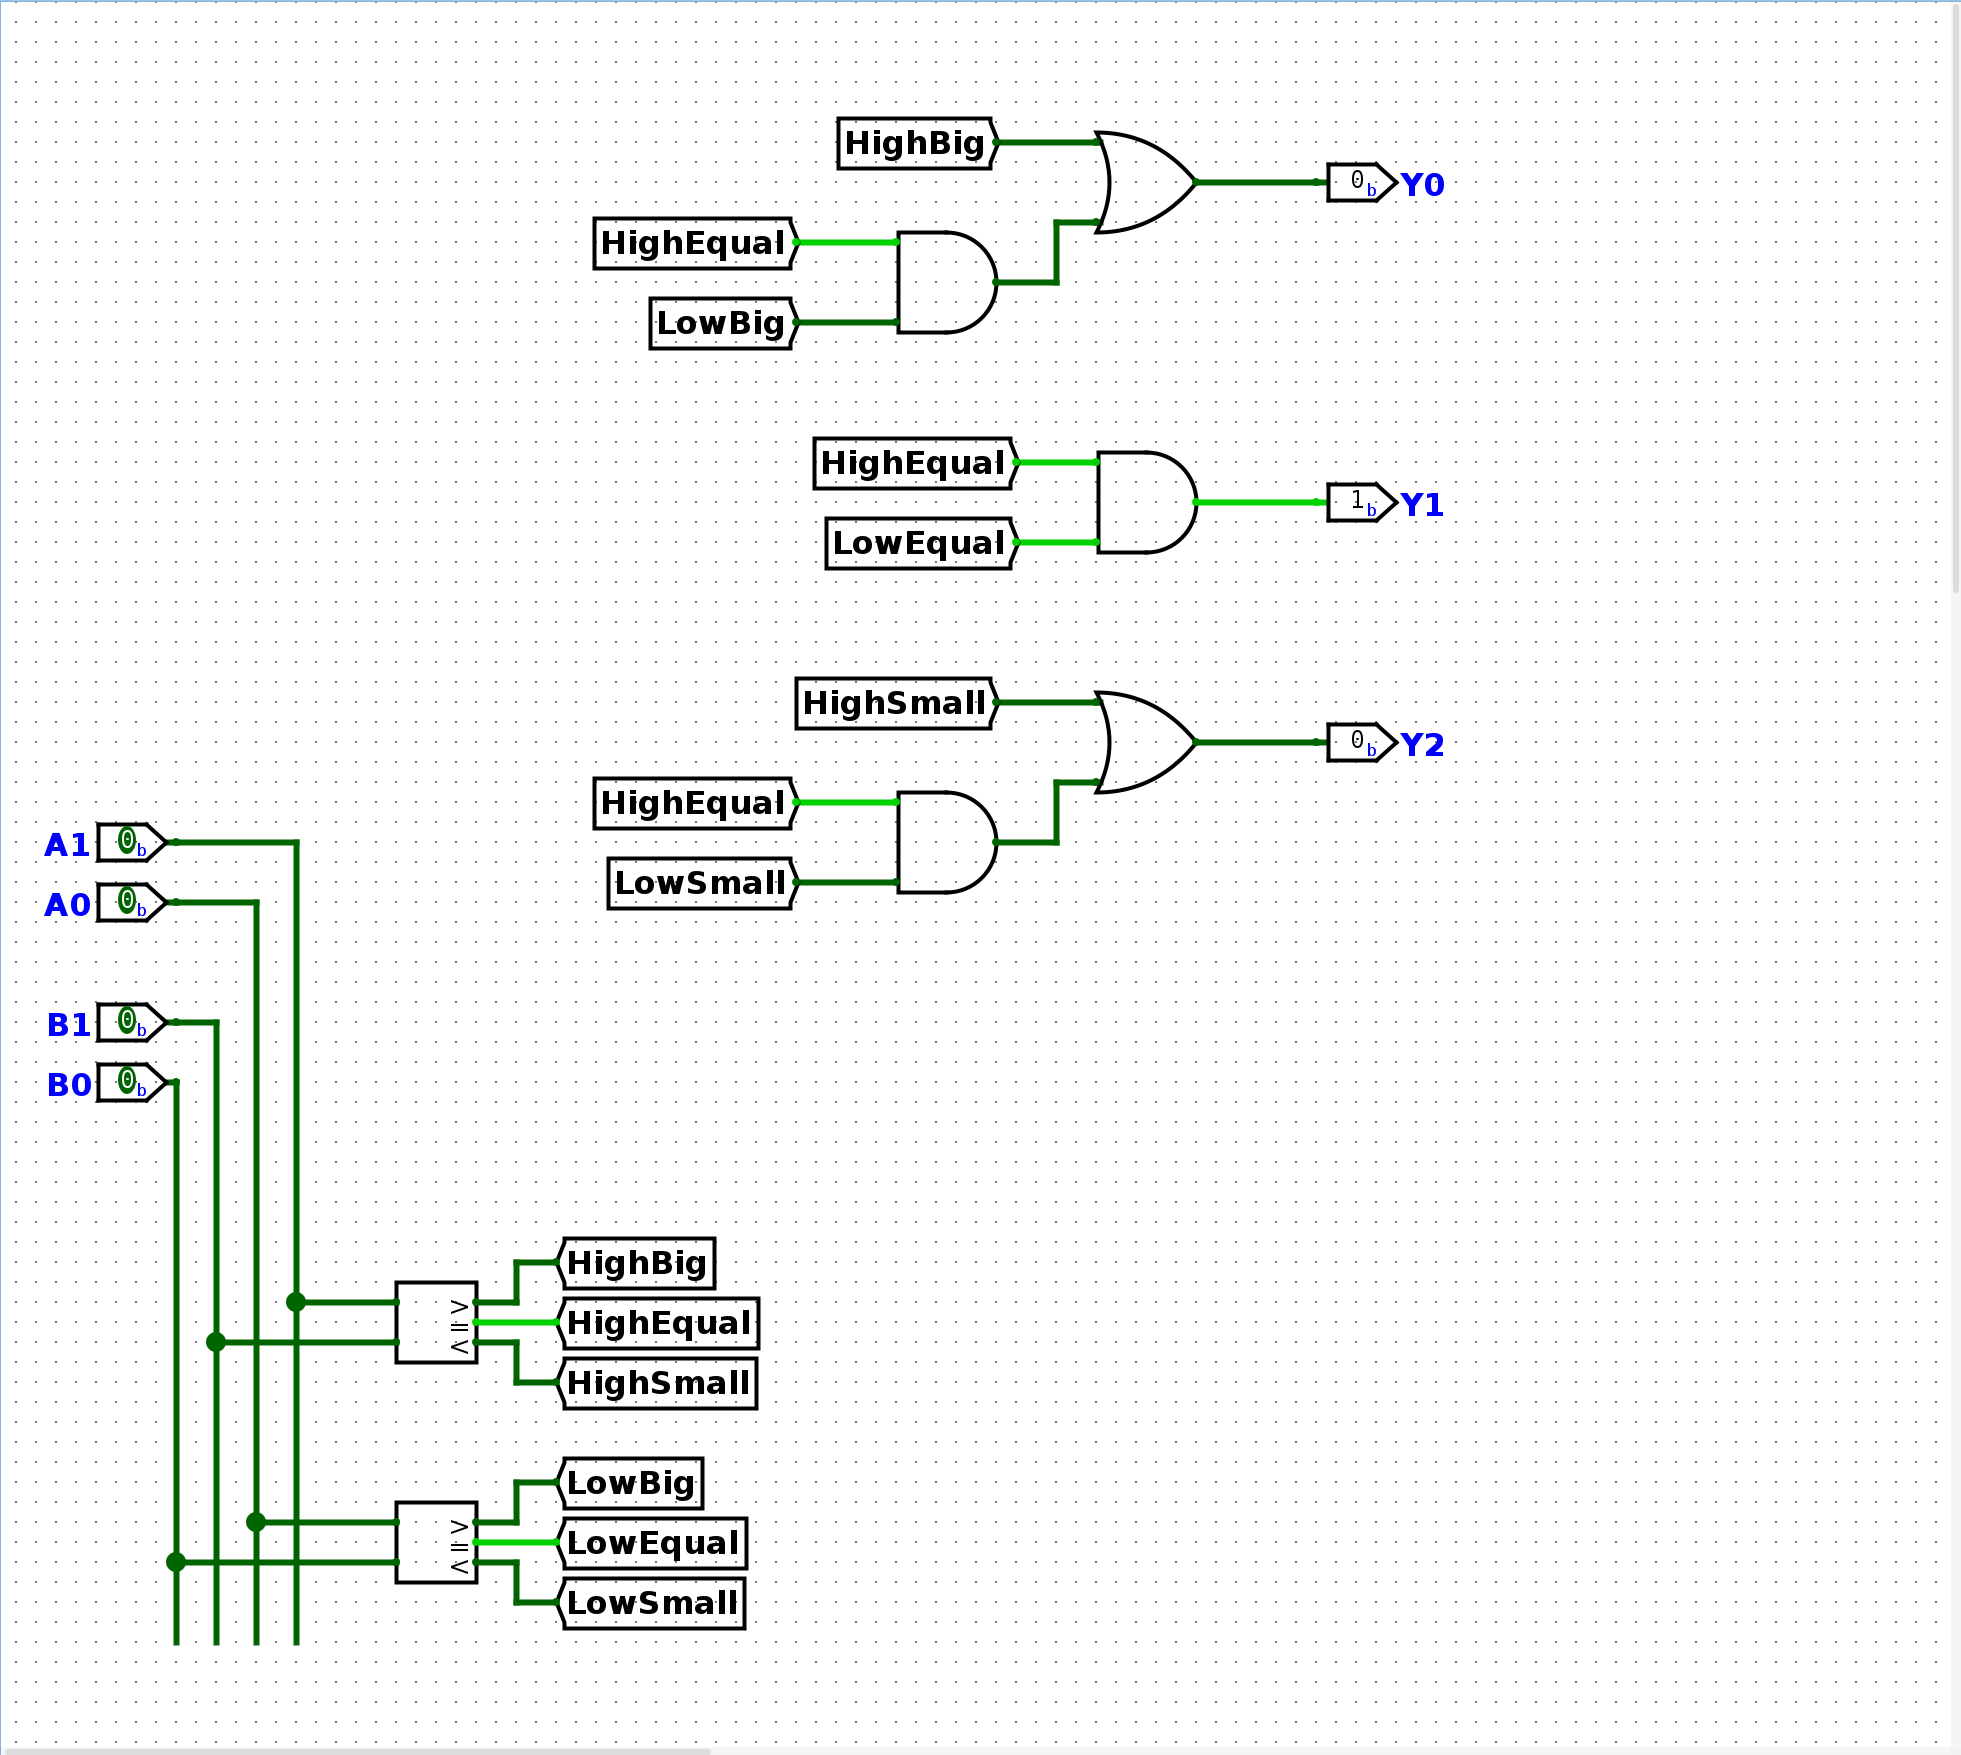
\includegraphics[width=0.95\textwidth]{Q1_comparator_2.png}


\end{answer}

\newpage
\section{SDS}
In the following circuit, NOT gates have a delay of 1ns, AND gates have a delay of 4ns, NAND gates have a delay of 3ns, OR gates have a delay of 4ns, NOR gates have a delay of 3ns. The registers have a clk-to-q delay of 2ns and setup time of 2ns. Assume the inputs
come from registers. All the delays refer to propagation delay.\\

\begin{figure}[hp]
    \centering
    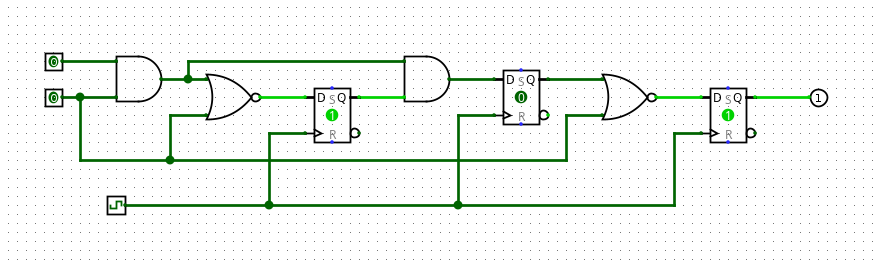
\includegraphics[width=1.0\textwidth]{Q2.png}
    \caption{Circuit Diagram}
    \label{fig:q2}
\end{figure}

What is the minimum acceptable clock cycle time for this circuit? What
clock frequency does it correspond to? (please include enough explanation) \textbf{[16 pt]}

\begin{answer}[Question 2]
    $t_1$ is the time from input to the first register. $t_2$ is the time from the first register to the second register. $t_3$ is the time from the second register to the third register. $t_4$ is the time from the third register to the output. The minimum clock cycle time is the maximum of these four times.
    \begin{align*}
        t_1       & = t_{clk-to-q} + t_{AND} + t_{NOR} + t_{setup} = 11 ns \\
        t_2       & = t_{clk-to-q} + 2 * t_{AND} + t_{setup} = 12ns        \\
        t_3       & = t_{clk-to-q} + t_{NOR} + t_{setup} = 7ns             \\
        t_4       & = t_{clk-to-q} = 2ns                                   \\
        t_{min}   & = max\{t_1, t_2, t_3, t_4\} = 12 ns                    \\
        f_{clock} & = \frac{1}{t_{min}} = \frac{1}{12ns} = 83.33MHz
    \end{align*}
\end{answer}

\newpage
\section{Finite state machine}
In this part, you need to implement a detector. When receiving two or more successive '0's or '1's, it outputs 1. For a bit sequence, it inputs one bit a period from left to right. e.g: input='11101001', output='01100010'.

(a) Draw the FSM (Moore machine) for this detector in five states: \{start\}, \{10\}(discrete '0'), \{01\}(discrete '1'), \{00\}(successive '0's), \{11\}(successive '1's). \\
e.g: input='011001', state=\{start\}$\xrightarrow{}$\{10\}$\xrightarrow{}$\{01\}$\xrightarrow{}$\{11\}$\xrightarrow{}$\{10\}$\xrightarrow{}$\{00\}$\xrightarrow{}$\{01\} \textbf{[10 pt]}

(b) Draw the FSM (Mealy machine) for this detector in no more than three states.\textbf{[10 pt]}

(c) Assign '000' to represent state \{start\}, '110' to represent \{10\}, '101' to represent \{01\}, '100' to represent \{00\}, '111' to represent \{11\}. We use 'CS' to represent current state and 'NS' for next state. Fill the truth table for the next-state and output logic based on the Moore FSM. \textbf{[15 pt]}

(d) Draw the circuit diagram for NS and output. \textbf{[15 pt]}
\begin{answer}[Question 3]
    (a)

    \begin{center}
        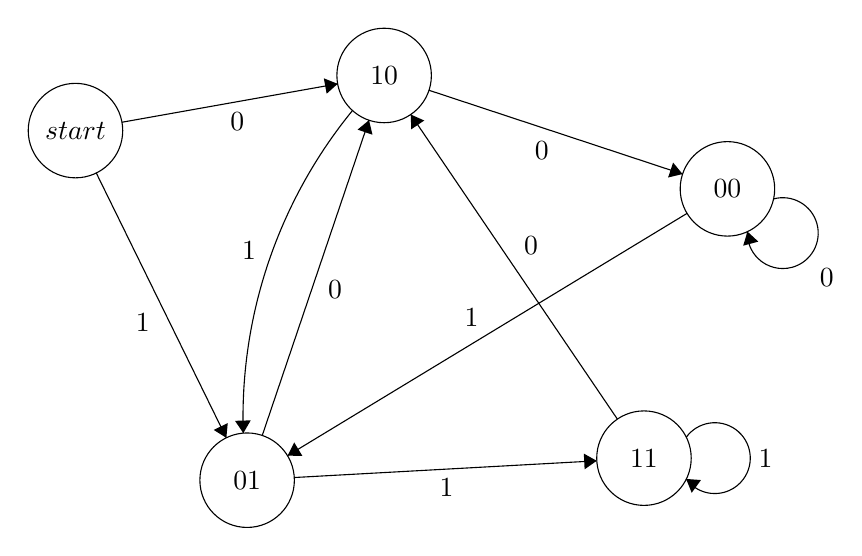
\begin{tikzpicture}[scale=0.2]
            \tikzstyle{every node}+=[inner sep=0pt]
            \draw [black] (17.4,-18.1) circle (3);
            \draw (17.4,-18.1) node {$start$};
            \draw [black] (37,-14.6) circle (3);
            \draw (37,-14.6) node {$10$};
            \draw [black] (28.3,-40.3) circle (3);
            \draw (28.3,-40.3) node {$01$};
            \draw [black] (58.8,-21.8) circle (3);
            \draw (58.8,-21.8) node {$00$};
            \draw [black] (53.5,-38.9) circle (3);
            \draw (53.5,-38.9) node {$11$};
            \draw [black] (20.35,-17.57) -- (34.05,-15.13);
            \fill [black] (34.05,-15.13) -- (33.17,-14.78) -- (33.35,-15.76);
            \draw (27.68,-16.94) node [below] {$0$};
            \draw [black] (18.72,-20.79) -- (26.98,-37.61);
            \fill [black] (26.98,-37.61) -- (27.07,-36.67) -- (26.18,-37.11);
            \draw (22.15,-30.29) node [left] {$1$};
            \draw [black] (28.055,-37.311) arc (-178.11616:-219.28796:30.755);
            \fill [black] (28.06,-37.31) -- (28.53,-36.5) -- (27.53,-36.53);
            \draw (28.9,-25.72) node [left] {$1$};
            \draw [black] (29.26,-37.46) -- (36.04,-17.44);
            \fill [black] (36.04,-17.44) -- (35.31,-18.04) -- (36.26,-18.36);
            \draw (33.41,-28.17) node [right] {$0$};
            \draw [black] (39.85,-15.54) -- (55.95,-20.86);
            \fill [black] (55.95,-20.86) -- (55.35,-20.13) -- (55.03,-21.08);
            \draw (47.01,-18.74) node [below] {$0$};
            \draw [black] (31.3,-40.13) -- (50.5,-39.07);
            \fill [black] (50.5,-39.07) -- (49.68,-38.61) -- (49.73,-39.61);
            \draw (40.96,-40.15) node [below] {$1$};
            \draw [black] (51.81,-36.42) -- (38.69,-17.08);
            \fill [black] (38.69,-17.08) -- (38.72,-18.02) -- (39.55,-17.46);
            \draw (45.85,-25.4) node [right] {$0$};
            \draw [black] (56.23,-23.36) -- (30.87,-38.74);
            \fill [black] (30.87,-38.74) -- (31.81,-38.76) -- (31.29,-37.9);
            \draw (42.55,-30.55) node [above] {$1$};
            \draw [black] (61.719,-22.441) arc (105.34019:-182.65981:2.25);
            \draw (64.63,-27.44) node [right] {$0$};
            \fill [black] (60.07,-24.51) -- (59.8,-25.41) -- (60.76,-25.15);
            \draw [black] (56.18,-37.577) arc (144:-144:2.25);
            \draw (60.75,-38.9) node [right] {$1$};
            \fill [black] (56.18,-40.22) -- (56.53,-41.1) -- (57.12,-40.29);
        \end{tikzpicture}
    \end{center}

    (b)

    \begin{center}
        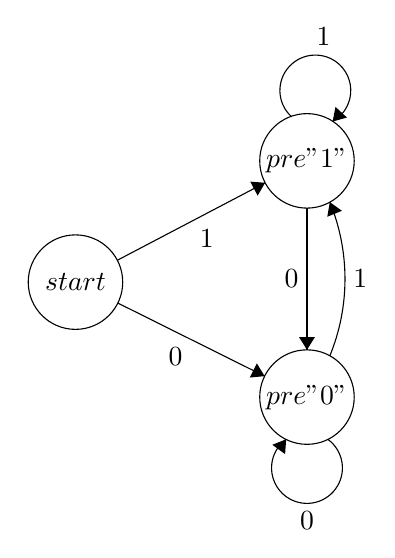
\begin{tikzpicture}[scale=0.2]
            \tikzstyle{every node}+=[inner sep=0pt]
            \draw [black] (21.5,-27.6) circle (3);
            \draw (21.5,-27.6) node {$start$};
            \draw [black] (36.2,-19.9) circle (3);
            \draw (36.2,-19.9) node {$pre"1"$};
            \draw [black] (36.2,-34.9) circle (3);
            \draw (36.2,-34.9) node {$pre"0"$};
            \draw [black] (24.16,-26.21) -- (33.54,-21.29);
            \fill [black] (33.54,-21.29) -- (32.6,-21.22) -- (33.07,-22.11);
            \draw (29.84,-24.25) node [below] {$1$};
            \draw [black] (24.19,-28.93) -- (33.51,-33.57);
            \fill [black] (33.51,-33.57) -- (33.02,-32.76) -- (32.57,-33.66);
            \draw (27.86,-31.75) node [below] {$0$};
            \draw [black] (37.651,-22.518) arc (22.31499:-22.31499:12.858);
            \fill [black] (37.65,-22.52) -- (37.49,-23.45) -- (38.42,-23.07);
            \draw (39.11,-27.4) node [right] {$1$};
            \draw [black] (36.2,-22.9) -- (36.2,-31.9);
            \fill [black] (36.2,-31.9) -- (36.7,-31.1) -- (35.7,-31.1);
            \draw (35.7,-27.4) node [left] {$0$};
            \draw [black] (35.203,-17.083) arc (227.22087:-60.77913:2.25);
            \draw (37.25,-12.61) node [above] {$1$};
            \fill [black] (37.83,-17.4) -- (38.74,-17.15) -- (38.01,-16.47);
            \draw [black] (37.523,-37.58) arc (54:-234:2.25);
            \draw (36.2,-42.15) node [below] {$0$};
            \fill [black] (34.88,-37.58) -- (34,-37.93) -- (34.81,-38.52);
        \end{tikzpicture}
    \end{center}

    (c) Do not modify the given values in the truth table.\\
    \begin{center}
        \begin{tabular}{ |c|c|c|c||c|c|c|c| }
            \hline
            CS[2] & CS[1] & CS[0] & input & NS[2] & NS[1] & NS[0] & output \\
            \hline
            0     & 0     & 0     & 0     & 1     & 1     & 0     & 0      \\
            \hline
            0     & 0     & 0     & 1     & 1     & 0     & 1     & 0      \\
            \hline
            1     & 1     & 0     & 0     & 1     & 0     & 0     & 1      \\
            \hline
            1     & 1     & 0     & 1     & 1     & 0     & 1     & 0      \\
            \hline
            1     & 0     & 1     & 0     & 1     & 1     & 0     & 0      \\
            \hline
            1     & 0     & 1     & 1     & 1     & 1     & 1     & 1      \\
            \hline
            1     & 0     & 0     & 0     & 1     & 0     & 0     & 1      \\
            \hline
            1     & 0     & 0     & 1     & 1     & 0     & 1     & 0      \\
            \hline
            1     & 1     & 1     & 0     & 1     & 1     & 0     & 0      \\
            \hline
            1     & 1     & 1     & 1     & 1     & 1     & 1     & 1      \\
            \hline
        \end{tabular}
    \end{center}

    (d)

    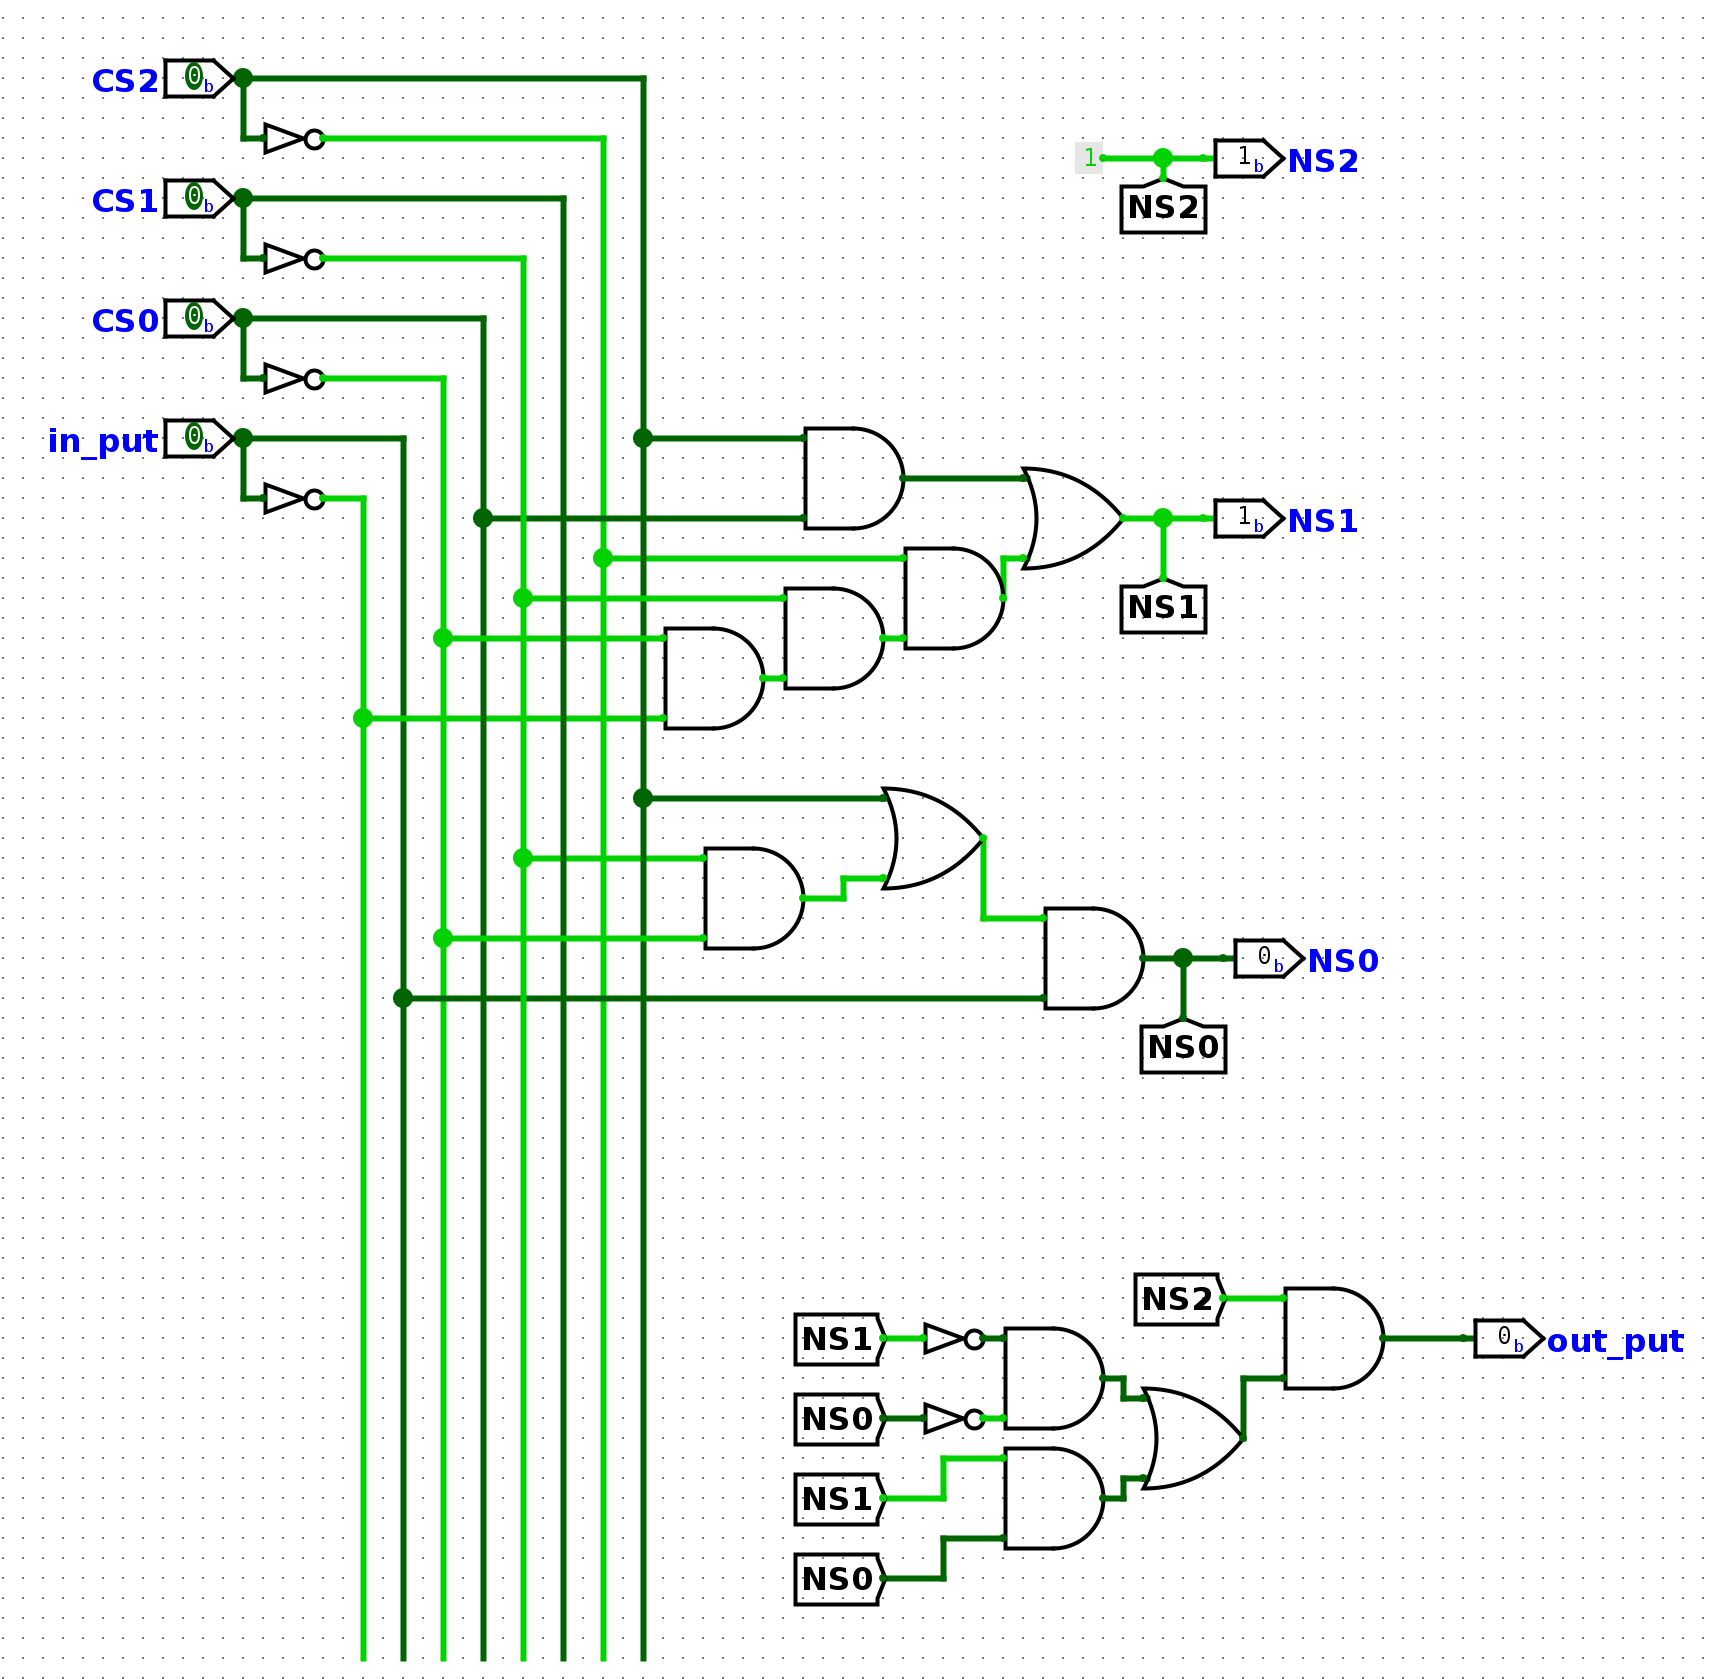
\includegraphics[width=0.95\textwidth]{Q3.png}

\end{answer}

\end{document}
